\chapter{Definire needs, tasks e storyboards}
\section{Task analysis}
Il Task Analysis è un metodo di analisi usato per comprendere come gli utenti eseguono determinate attività, con l’obiettivo di progettare sistemi interattivi che rispondano efficacemente ai loro bisogni. Questo processo consente di raccogliere informazioni su ciò che gli utenti fanno, quali strumenti utilizzano e come raggiungono i loro obiettivi, aiutando i progettisti a sviluppare interfacce più intuitive e mirate.

Nel processo di progettazione centrata sull'utente, il Task Analysis è un passaggio intermedio tra l’analisi dei bisogni dell’utente e il design dell’interfaccia. Serve a rendere espliciti i bisogni degli utenti e a rappresentare i risultati dell’analisi in modo chiaro. Nel processo, i bisogni vengono tradotti in obiettivi concreti, che a loro volta si trasformano in azioni. Un esempio pratico potrebbe essere il bisogno di "migliorare il benessere", che si traduce nell'obiettivo di "fare esercizio fisico regolarmente" o "monitorare il sonno", e infine nelle azioni di utilizzare app per il monitoraggio delle attività fisiche o del sonno. Tuttavia, il contesto influisce sugli obiettivi, ma non sui bisogni di fondo. Ad esempio, il bisogno di "sentirsi sicuri" può tradursi in un obiettivo come "ottenere una promozione" o "installare un sistema di sicurezza a casa", a seconda del contesto.

Il Task Analysis è lo studio di come le persone svolgono le loro attività quotidiane. L’obiettivo principale è determinare:
\begin{enumerate}
    \item \textit{Cosa fanno:} quali sono i passaggi necessari per completare un'attività.
    \item \textit{Quali strumenti usano:} gli artefatti che impiegano per svolgere le attività.
    \item \textit{Quanto bene riescono a completare l'attività:} quali sono i loro obiettivi e quanto successo hanno nel raggiungerli.
\end{enumerate}
Secondo Benyon, \textit{"un task è definito come un obiettivo accompagnato da una serie ordinata di azioni necessarie per raggiungerlo"}. Esistono diversi livelli di astrazione per descrivere un task:
\begin{itemize}
    \item \textit{Goal:} lo stato che l'utente vuole raggiungere.
    \item \textit{Task:} un insieme strutturato di attività necessarie per raggiungere il goal usando una specifica tecnologia.
    \item \textit{Action:} un task semplice che non richiede risoluzione di problemi o controllo.
\end{itemize}

\begin{figure}[ht]
    \centering
    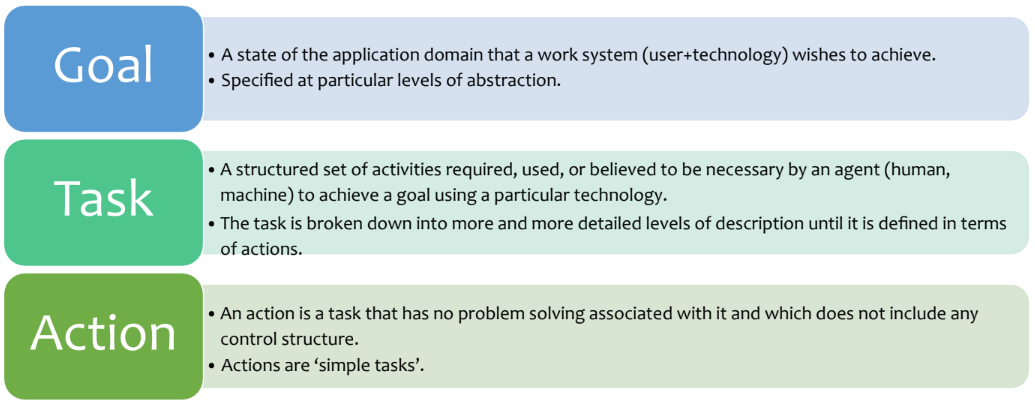
\includegraphics[width=0.7\linewidth]{images/goal-task.PNG}
    \caption{Goal, task e action}
    \label{fig:enter-label}
\end{figure}

Attraverso l’analisi dei task, si ottengono informazioni dettagliate su cosa gli utenti cercano di ottenere, come eseguono i task e quali esperienze personali, sociali e culturali influenzano il loro lavoro. Si apprende anche come l'ambiente fisico e l'esperienza pregressa influenzino il workflow degli utenti e i punti di difficoltà che incontrano.

Tuttavia, una delle principali sfide è che i progettisti non creano i task, bensì le interfacce. Questo significa che i task e gli oggetti non hanno sempre una corrispondenza uno-a-uno. Ad esempio, un'applicazione web può supportare molteplici task diversi, e le persone possono usare la stessa interfaccia per ottenere risultati leggermente differenti o per eseguire attività diverse.

\begin{Example}{Uber}{}
\textit{Esaminiamo un servizio come Uber.} 

Gli utenti di Uber possono avere diversi bisogni:
\begin{enumerate}
    \item \textit{Necessità di un trasporto rapido o sicuro:} l'utente desidera un modo rapido e semplice per andare dal punto A al punto B senza la seccatura di cercare un mezzo pubblico o di guidare da solo.
    
    Un task associato al bisogno di trasporto conveniente potrebbe essere quello di "richiedere un'auto attraverso l'app". In questo caso, l'interfaccia permette all'utente di scegliere un punto di partenza e una destinazione, trovando un autista disponibile nelle vicinanze.

    \item \textit{Necessità di sicurezza durante il viaggio:} l'utente desidera sentirsi al sicuro durante il viaggio, sia tramite conducenti controllati, monitoraggio in tempo reale o assicurandosi che qualcuno conosca la sua posizione. 
    
    Il task associato potrebbe consistere nel "verificare i dettagli del conducente e monitorare il progresso del viaggio". L'app fornisce informazioni sull'identità e i dettagli del veicolo del conducente, e consente all'utente di tracciare la posizione del veicolo in tempo reale.

    \item \textit{Necessità di trasporto conveniente:} l'utente desidera bilanciare la comodità con l'accessibilità economica e assicurarsi di ottenere un viaggio a un prezzo ragionevole. 

    Il task sarebbe "valutare le opzioni di trasporto in base al costo e alla disponibilità". L'app permette di confrontare diverse opzioni (come corse condivise o private) e fornisce stime di costo, consentendo all'utente di scegliere l'opzione che meglio si adatta al suo budget.
\end{enumerate}
\end{Example}

\section{Personas}
Nel design dell'Interazione Uomo-Macchina (HCI), uno degli strumenti più utili per migliorare la progettazione delle interfacce è il concetto di \textit{personas}. Le personas rappresentano modelli astratti di utenti reali, basati su dati concreti, e vengono create per comprendere meglio le esigenze e i comportamenti degli utenti durante il processo di design.

Una persona non è semplicemente una caricatura di un utente generico, ma una rappresentazione semi-fittizia che si basa su dati demografici, comportamentali e psicografici reali. Queste informazioni permettono ai progettisti di modellare i diversi tipi di utenti con cui dovranno interagire. L’obiettivo è quello di suddividere gli utenti in categorie con caratteristiche, obiettivi e necessità specifiche, creando un'immagine dettagliata che diventi un riferimento per tutto il team di progettazione.

Le personas aiutano i progettisti a mettersi nei panni degli utenti reali, creando empatia. Immaginare un utente concreto con desideri, bisogni e frustrazioni, permette ai designer di comprendere meglio il punto di vista degli utenti. Questo processo facilita anche il miglioramento dell'esperienza utente (UX), in quanto le personas diventano uno strumento guida per le decisioni di design. Quando i progettisti si trovano a dover scegliere tra diverse soluzioni, possono chiedersi cosa preferirebbe una determinata persona, aiutando a ottimizzare il prodotto per il target specifico.
Le personas forniscono anche un quadro di riferimento che aiuta a identificare esigenze e sfide degli utenti, creando così un focus più preciso nella progettazione. Questo è particolarmente utile quando ci si rende conto che non è possibile progettare un'interfaccia che vada bene per tutti, poiché si rischierebbe di non soddisfare pienamente nessuno.

Ogni persona è composta da diversi elementi chiave che forniscono una rappresentazione completa dell’utente:
\begin{enumerate}
    \item \textit{Nome:} Dare un nome alla persona rende l'utente più umano e più facile da visualizzare per il team di progettazione.
    \item \textit{Foto:} Un'immagine rafforza l'identità della persona, rendendo l'utente fittizio più reale e favorendo un maggiore coinvolgimento emotivo da parte dei progettisti.
    \item \textit{Caratteristiche demografiche:} Età, genere, professione e livello di istruzione sono tutti dati essenziali per comprendere meglio il background dell'utente e il modo in cui potrebbe interagire con il sistema.
    \item \textit{Obiettivi:} Cosa vuole ottenere l'utente utilizzando l'interfaccia? Ad esempio, potrebbe voler completare rapidamente un'azione o potrebbe cercare di esplorare nuove funzionalità.
    \item \textit{Frustrazioni:} Quali sono i principali problemi che l'utente potrebbe incontrare durante l'uso del sistema? Questi possono includere difficoltà tecniche o sfide specifiche legate alla comprensione dell'interfaccia.
    \item \textit{Comportamenti:} Le abitudini e il modo in cui l'utente interagisce con il sistema sono cruciali per progettare soluzioni che siano intuitive e in linea con le aspettative.
\end{enumerate}
L'uso delle personas porta numerosi vantaggi nel processo di progettazione delle interfacce. Uno dei benefici principali è che aiutano i designer a creare empatia con l'utente. Interiorizzando gli obiettivi e i bisogni dell'utente fittizio, i progettisti possono prendere decisioni più accurate, basate su una visione concreta di chi utilizzerà il prodotto.
Un altro vantaggio è la capacità di sviluppare un focus: le personas rendono chiaro che non è possibile progettare per tutti. Concentrarsi su utenti specifici permette di evitare un design troppo generico e privo di personalità. Inoltre, le personas aiutano a comunicare le conclusioni della ricerca, condividendo intuizioni e risultati con coloro che non hanno partecipato direttamente agli incontri con gli utenti, come stakeholder e altri membri del team.
Le personas facilitano anche il processo decisionale, in quanto permettono di vedere il mondo dalla prospettiva dell'utente, rendendo più semplice determinare quali funzionalità sono utili e quali potrebbero essere casi limite. Inoltre, possono fungere da sostituti degli utenti durante la fase di test, aiutando a misurare l'efficacia delle soluzioni proposte.

\section{Storyboards}
Nel campo dell'Interazione Uomo-Macchina (HCI), gli \textit{storyboards} rappresentano un potente strumento di comunicazione visiva utilizzato per raffigurare l'aspetto esteriore di un sistema, senza mostrare le sue funzionalità interne. Sono spesso utilizzati come supporto per illustrare come si svolgono i task da parte degli utenti, il contesto in cui l'utente utilizzerà il sistema, i passaggi principali del task e l'interazione tra gli utenti e l'ambiente. Vengono rappresentati in forma di fumetti disegnati a mano, con una sequenza di sketch che rappresentano i passaggi chiave di un'azione.

Uno storyboard è una rappresentazione grafica che mostra come una persona può portare a termine un task attraverso l'interazione con un sistema o un'interfaccia. La sua natura "fumettistica" rende il processo immediato, permettendo ai progettisti di concentrarsi sul flusso del task, piuttosto che sui dettagli tecnici o visivi dell'interfaccia. Uno degli elementi distintivi degli storyboard è la presenza di persone: infatti, uno storyboard efficace deve sempre includere individui che interagiscono con l'interfaccia o tra di loro.

\begin{figure}[ht]
    \centering
    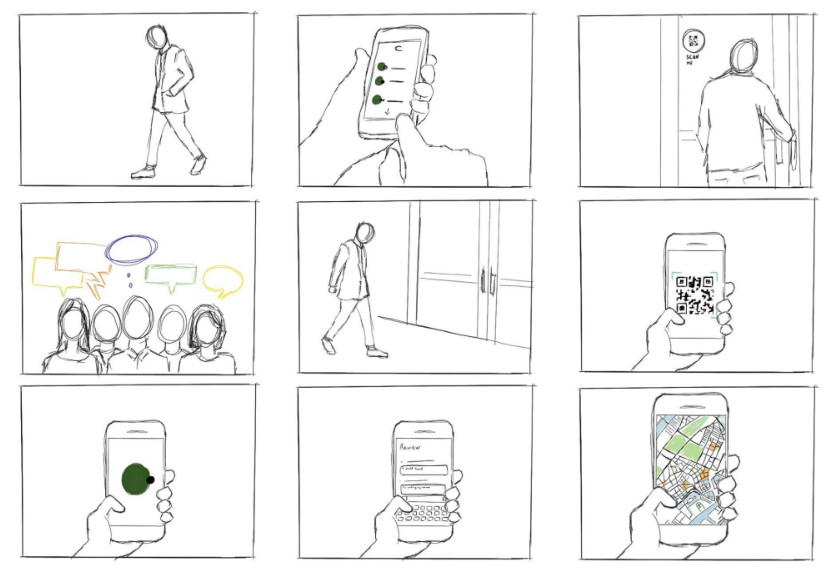
\includegraphics[width=0.5\linewidth]{images/storyboards.jpeg}
    \caption{Storyboards}
    \label{fig:storyboards}
\end{figure}

Uno degli aspetti più utili degli storyboard è la loro capacità di rappresentare cosa accade nei momenti chiave di un task, mostrando come un utente interagisce con il sistema in diverse fasi temporali. Non è richiesta alcuna particolare abilità artistica, poiché lo scopo principale non è creare immagini "belle", ma comunicare le idee. I progettisti devono quindi concentrarsi sul raccontare una storia e far emergere il contesto in cui si svolge l'interazione.

Uno storyboard efficace deve includere diversi aspetti fondamentali. Il primo è l'illustrazione di un obiettivo, ovvero cosa l'utente cerca di ottenere con il task rappresentato. Successivamente, deve mostrare come il task si sviluppa, cioè come l'utente interagisce con il sistema e con altre persone o dispositivi. Ogni passo significativo del task deve essere rappresentato in modo chiaro, fino a mostrare l'esito finale, che illustra come l'utente raggiunge il proprio obiettivo in modo soddisfacente.

È importante sottolineare che in questa fase non si dovrebbero ancora disegnare le schermate dell'interfaccia. Rappresentare già le schermate potrebbe vincolare troppo le decisioni sul design, mentre in questo momento l'obiettivo è comprendere come si sviluppano i task e come gli utenti interagiscono con il sistema.

\begin{Example}{Storyboard - Ricetta}{}
\textit{Immaginiamo uno storyboard che mostra una persona che utilizza un'app cercare una ricetta da preparare per cena.} 

Le prime immagini illustrano l'utente che finisce di lavorare, prende la metropolitana e prova a utilizzare l'app ma c'è assenza di segnale. Successivamente consulta la lista della spesa per acquistare gli ingredienti e, infine, prepara il pasto una volta a casa. 

\begin{minipage}{\textwidth}
    \centering
    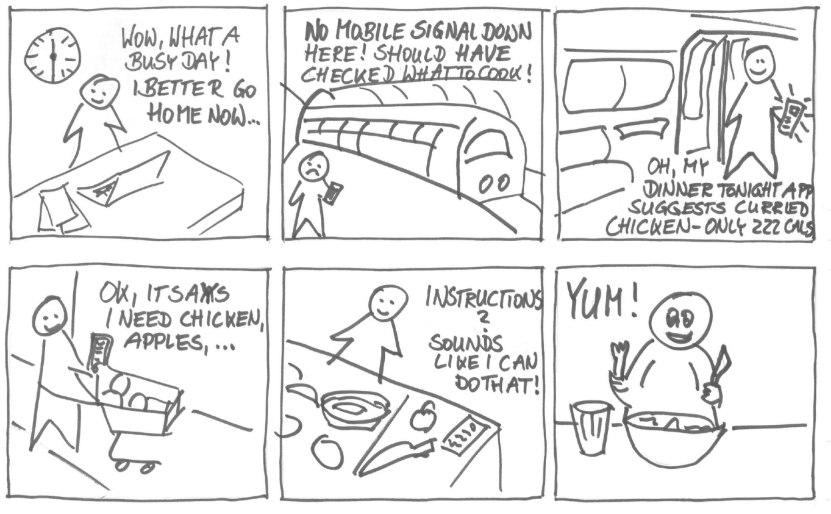
\includegraphics[width=0.6\textwidth]{images/storyboard-es1.jpeg}
    %\captionof{figure}{Esempio}
\end{minipage}

Lo storyboard ci permette di capire che l'utente vorrebbe usare l'applicazione anche quando c'è assenza di segnale. Inoltre riusciamo ad intuire che l'app dovrebbe consigliare una ricetta, mostrare le calorie, gli ingredienti e le istruzioni per prepararla.
\end{Example}

\begin{Example}{Storyboard - Cucina}{}
\textit{Questo storyboard mostra come un'app può convincere un utente che cucinare un pasto a casa sia più veloce rispetto a ordinare del cibo da asporto.} 

In questo caso, lo storyboard rappresenta l'interfaccia dell'app mentre mostra ricette con ingredienti che l'utente ha già nel frigorifero, rendendo la preparazione del pasto immediata.

\begin{minipage}{\textwidth}
    \centering
    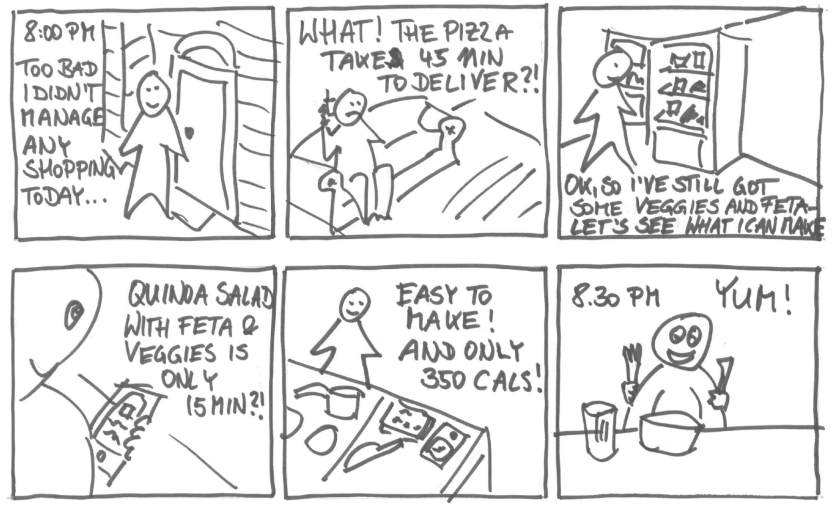
\includegraphics[width=0.6\textwidth]{images/storyboard-es2.jpeg}
    %\captionof{figure}{Esempio}
\end{minipage}
\end{Example}

Ogni storyboard dovrebbe riuscire a comunicare tre elementi principali: \textit{ambientazione}, \textit{sequenza} e \textit{soddisfazione}. L'ambientazione include i personaggi, ovvero le persone coinvolte, l'ambiente in cui si trovano e il compito che stanno svolgendo. La sequenza mostra i passaggi necessari per portare a termine il task, senza però soffermarsi sui dettagli tecnici dell'interfaccia utente. Il ruolo dell'interfaccia deve essere evidenziato come uno strumento che facilita il raggiungimento dell'obiettivo dell'utente.
Infine, lo storyboard deve trasmettere il concetto di soddisfazione, mostrando cosa motiva l'utente a completare il task e qual è il risultato finale che desidera ottenere. Questa parte è fondamentale, poiché sottolinea come il sistema o l'app rispondano a un bisogno reale dell'utente.

Esistono diversi tipi di storyboard, ognuno adatto a situazioni specifiche. Lo storyboard tradizionale segue convenzioni simili a quelle dei fumetti, con personaggi, nuvolette di dialogo e un sfondo che illustra l'ambiente. Spesso si aggiungono note a ogni scena per spiegare ciò che sta accadendo.
Quando l'interfaccia è molto dinamica o contiene elementi multimediali specifici, si possono usare scored storyboards, che includono annotazioni aggiuntive su movimenti, colori e suoni. Infine, nei casi in cui l'interazione è troppo complessa per essere rappresentata visivamente, si possono utilizzare storyboard testuali, che descrivono in modo dettagliato il comportamento dell'utente e del sistema.

Perché disegnare a mano? Disegnare uno storyboard a mano ha diversi vantaggi. È un metodo rapido, che non richiede tempo da dedicare a strumenti di grafica, i quali spesso spingono i progettisti a focalizzarsi troppo sui dettagli estetici piuttosto che sul flusso del task. La natura imprecisa del disegno a mano fa sì che gli utenti si sentano più liberi di esprimere commenti e suggerimenti, rispetto a versioni più "raffinate" o professionali, che possono scoraggiare il feedback.
Uno storyboard disegnato a mano permette inoltre ai progettisti di sperimentare rapidamente diverse soluzioni e scenari, senza la pressione di dover creare disegni perfetti o complessi. Gli utenti e i membri del team possono concentrarsi esclusivamente sul contenuto del task, senza essere distratti da font, colori o icone.

\begin{figure}[ht]
    \centering
    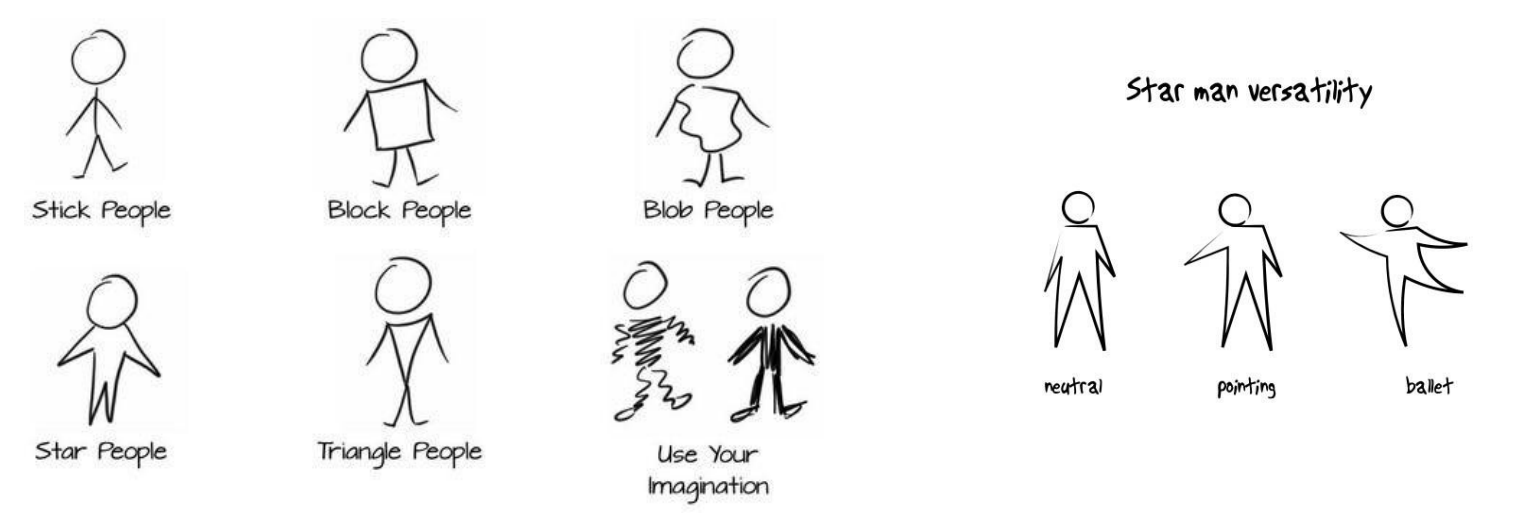
\includegraphics[width=0.8\linewidth]{images/sketching-people.PNG}
    \caption{Sketching people}
    \label{fig:sketching-people}
\end{figure}

Per una singola applicazione, di solito si crea uno storyboard per 1-2 task principali. È importante non cercare di rappresentare ogni possibile task, poiché un errore comune è voler fare troppo e includere ogni dettaglio. Una buona pratica è ridurre il numero di storyboard a un massimo di 3-5 task, il che di solito corrisponde a 2-4 storyboard per progetto. Questo approccio permette di mantenere il focus sui task più critici, senza perdere tempo su task secondari che potrebbero essere affrontati in seguito.

L'uso degli storyboard porta numerosi benefici nel processo di progettazione. Innanzitutto, enfatizzano come un'interfaccia aiuta a completare un task, mantenendo il focus della discussione sui compiti degli utenti, piuttosto che sui dettagli superficiali dell'interfaccia, come la posizione dei pulsanti. Gli storyboard sono un ottimo strumento per garantire che tutti i membri del team di progettazione abbiano una visione condivisa sugli obiettivi dell'app, evitando discussioni inutili su dettagli tecnici.